\chapter{Gitter (Lattices)}\label{ch:lattices}

\begin{figure}[H]
    \centering
    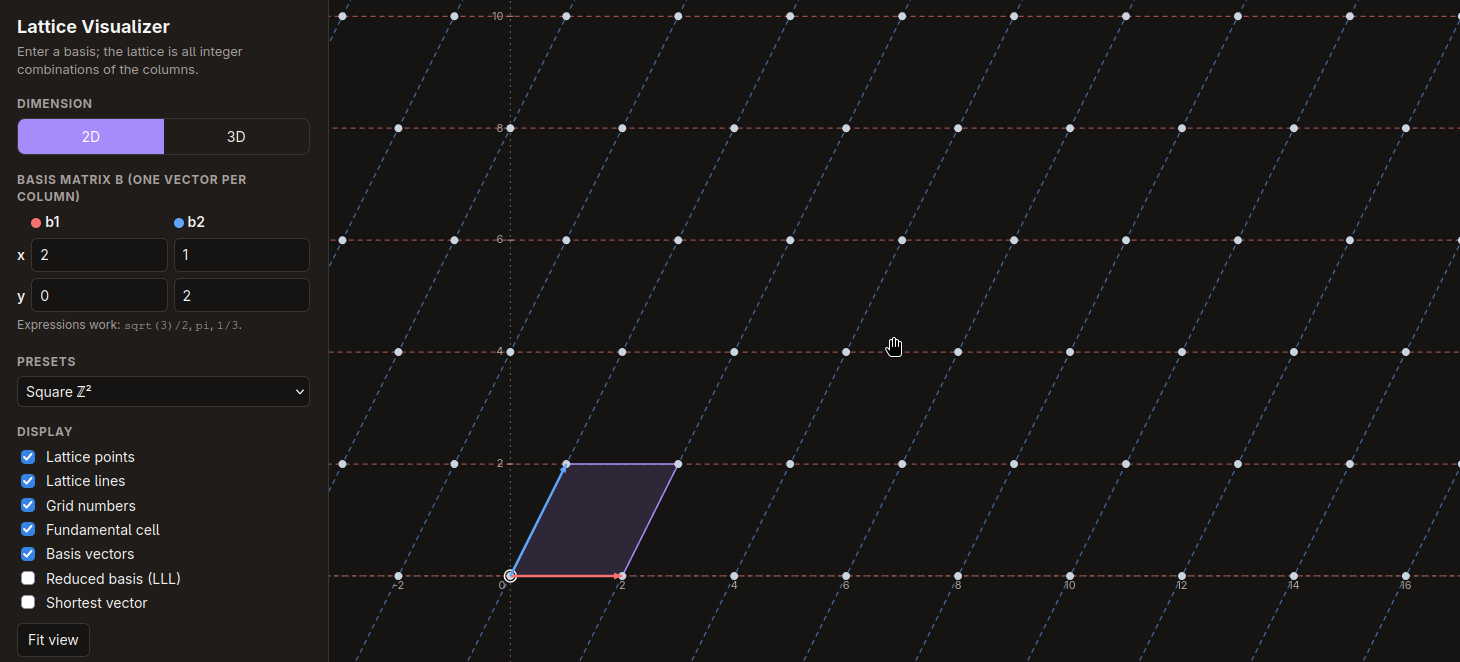
\includegraphics[width=0.9\textwidth]{../assets/lattice_tool_simple_2d_lattice.png}
    \caption{Ein einfaches zweidimensionales Gitter}
\end{figure}

Gitter sind im kryptografischen Kontext interessant, weil eine günstige Basis einige Berechnungen stark vereinfacht, während dieselbe Berechnung mit einer schlechten Basis fast unmöglich sein kann.

\section{Grundlagen}
Ein \textbf{euklidischer Vektorraum} ist ein reeller Vektorraum mit einem Skalarprodukt, zum Beispiel die Ebene $\mathbb{R}^2$ mit $\langle \mathbf{u}, \mathbf{v} \rangle = u_1 v_1 + u_2 v_2$.

Vektoren $\mathbf{b}_1, \dots, \mathbf{b}_m$ sind \textbf{linear unabhängig}, wenn aus $\sum_i a_i \mathbf{b}_i = \mathbf{0}$ folgt, dass alle $a_i = 0$ sind. Die Vektoren $\mathbf{b}_1 = (2, 1)^T$ und $\mathbf{b}_2 = (1, 3)^T$ sind unabhängig. Die Vektoren $(2, 1)^T$ und $(4, 2)^T$ sind abhängig, denn $\mathbf{b}_2 = 2\mathbf{b}_1$ und damit $2\mathbf{b}_1 - \mathbf{b}_2 = \mathbf{0}$.

\newpage

\section{Definition}
\begin{definition}[Gitter]
    Sei $B = \{\mathbf{b}_1, \mathbf{b}_2, \dots, \mathbf{b}_m\}$ eine Menge linear unabhängiger Vektoren aus dem euklidischen Vektorraum $\mathbb{R}^n$. Die Menge aller ganzzahligen Linearkombinationen
    \[
        \mathcal{L}(B) = \left\{ \sum_{i=1}^{m} a_i \mathbf{b}_i \;\middle|\; a_i \in \mathbb{Z} \right\} \subseteq \mathbb{R}^n
    \]
    heisst das von $B$ erzeugte \textbf{Gitter} in $\mathbb{R}^n$. $B$ nennt man die \textbf{Basis} des Gitters.
\end{definition}

Ein Gitter lässt sich auch aus einer Matrix $\mathbf{B}$ erzeugen, deren Spalten die Basisvektoren sind. Für die Basis $\{(2, 0)^T, (1, 2)^T\}$ ist
\[
    \mathbf{B} = \begin{pmatrix} 2 & 1 \\ 0 & 2 \end{pmatrix}
    \qquad\text{und}\qquad
    \mathcal{L}(\mathbf{B}) = \left\{ \mathbf{B}\mathbf{a} \;\middle|\; \mathbf{a} \in \mathbb{Z}^2 \right\}.
\]

\section{Eigenschaften}
\begin{itemize}
    \item Der \textbf{Rang} $m$ ist die Anzahl der Basisvektoren, die \textbf{Dimension} $n$ ist die Dimension des umgebenden Raums $\mathbb{R}^n$. Gilt $m = n$, heisst das Gitter \textbf{vollrangig}.
    \item Ein Gitter hat \textbf{viele Basen}. Dasselbe Gitter kann also auf verschiedene Arten beschrieben werden.
    \item Eine \textbf{gute Basis} besteht aus kurzen, fast orthogonalen Vektoren (Winkel nahe $90^\circ$).
    \item Eine \textbf{schlechte Basis} besteht aus langen, fast parallelen Vektoren (Winkel nahe $0^\circ$ oder $180^\circ$). Sie ist \glqq beinahe linear abhängig\grqq. Sind die Vektoren genau parallel, bilden sie gar keine Basis.
\end{itemize}

\begin{figure}[H]
    \centering
    \begin{subfigure}{0.48\textwidth}
        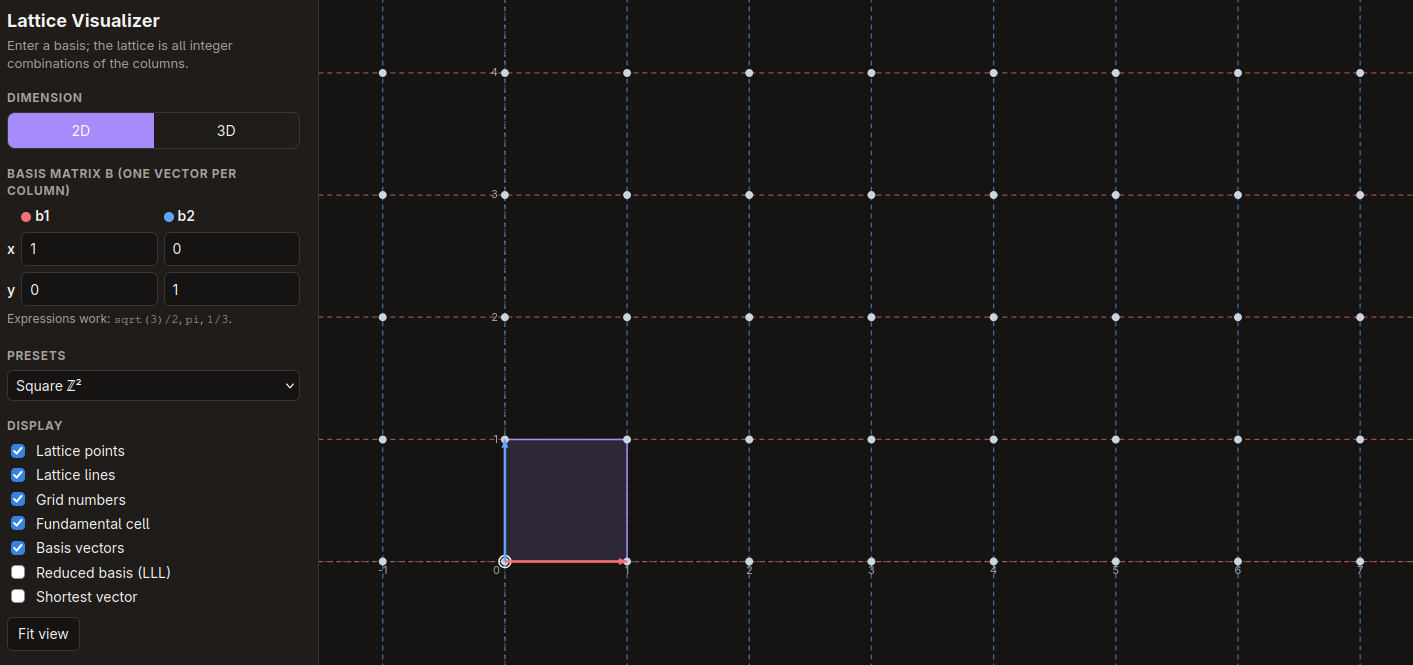
\includegraphics[width=\textwidth]{../assets/lattice_tool_good_basis.png}
        \caption{Gute Basis}
    \end{subfigure}
    \hfill
    \begin{subfigure}{0.48\textwidth}
        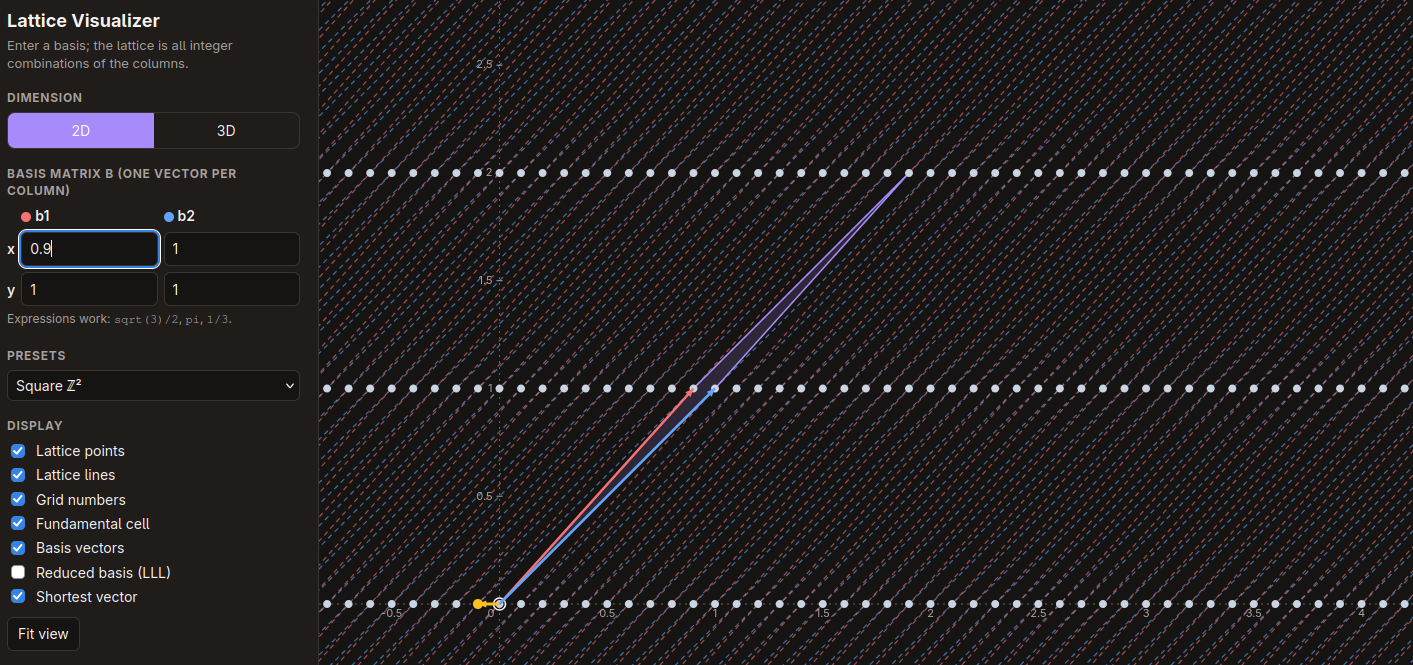
\includegraphics[width=\textwidth]{../assets/lattice_tool_bad_basis.png}
        \caption{Schlechte Basis}
    \end{subfigure}
    \caption{Zwei Basen desselben Gitters}
\end{figure}
